%
\subsection{Remote Client}
\label{sec:remote-cli-decomp}
%
In this section the remote client is analyzed, considering its events, use cases, dynamic operation and the flow of events.

\subsubsection{User mockups}
\label{sec:user-mockups-1}
%
In Fig.~\ref{fig:user-mockups-rc} is illustrated the user mockups for the remote client. 
It intends to clarify how does the~\gls{ui} works for the two different sides: Brands and Company (staff).

The initial state of the~\gls{mdo-rc}'s~\gls{ui} is depicted in thick border outline: the 'Sign In' window. 
If the \texttt{User} makes a mistake in its username and/or password, it will be shown an error message. 
Also, the 'Sign In' window has an option to recover the password, which sends an e-mail to switch password.
If the \texttt{User} still remembers its credentials, the app flows through one out of two possibilities: if the user is an admin, goes to the admin main menu, or else if the user is a brand, it will appear the brand main menu.

Firstly, the \texttt{Admin} workflow:
%
\begin{itemize}
\item The \texttt{Admin} main menu contains a drop down button with all the stations available. Choosing one of them, the \texttt{Admin} can turn it On/Off, see it's current mode and the current brand ad being displayed. Also, the \texttt{Admin}  can log out and choose between two different paths:
%
\begin{itemize}
\item \emph{Statistics}: It is possible to see various statistics of all different brands that are currently playing on the station: the number of times that the ad was shown, the number of pictures/\gls{gif}s and shared posts, the fragrance slot and quantity (percentage) and the days remaining for the rent to end.
It is also possible to deactivate the add if something wrong occurs and go back to the previous menu.
\item \emph{Users}: In this window, the admin can manage all users and see their information.
It is possible to the admin to change the type of user to brand or to admin, and it can also remove its type.
Also, the admin can delete users from the database. 
\item \emph{Ads to Activate}: In this window, the \texttt{Admin} can handle all the ads that the brands are intending to rent.
For that, the \texttt{Admin} needs to see if everything is in order, such as if all the videos that the brand wants to display are in order (in case there are some  or decontextualized videos), if it has a filter, a fragrance and a slot.
After that, the \texttt{Admin} can either accept or deny the ad.
If it accepts the ad, it is shown a success message and the ad is added to the station with its preferences.
If the ad is denied, the \texttt{Admin} needs to send a reason why it denied the ad, that is consequently send to the brand's email.
\end{itemize}
%
\end{itemize}

Secondly, the \texttt{Brand} workflow:
\begin{itemize}
\item The \texttt{Brand} main menu contains a welcome message, a notification bell to see if another ad was accepted or denied and three buttons - Rented, To Rent and Log Out.
The 'Log Out' button logs the \texttt{Brand} out of its account, the other two buttons switch to different widgets:
%
\begin{itemize}
\item \emph{Rented}: The \texttt{Brand} can see all statistics of all its rented ads on different stations that it rented.
That statistics are: status, number of times the ad was shown, the fragrance slot and quantity (percentage), the number of pictures/\gls{gif}s taken, the number of shared posts and the number of days remaining to end its rent.
The 'Go Back' button goes back to the previous menu.
\item \emph{To Rent}: The \texttt{Brand} can rent ads in the same station or in other stations.
To that happens, it is only needed to choose the target hours and then a calendar will show what days are available to that hours, then after choosing the days, the \texttt{Brand} need to upload a filter and a .zip file with a maximum of ten videos. 
Finally, the \texttt{Brand} needs to select the fragrance that wants to spill to the air and select 'Rent'. After that, a success message will be shown and the ad will enter in wait list for an \texttt{Admin} check if everything is in order.
\end{itemize}
%
\end{itemize}

It is also possible to register a new user through the 'Register' button.
This opens a window to type a username, a password, confirm the password and the e-mail.
If everything is in order, the user is created with the default user type of Brand.

Finally, at any time, it can occur the loss of internet connection, which toggles an error message informing the automatic log out of the account.
\begin{figure}[htb!]
\centering
    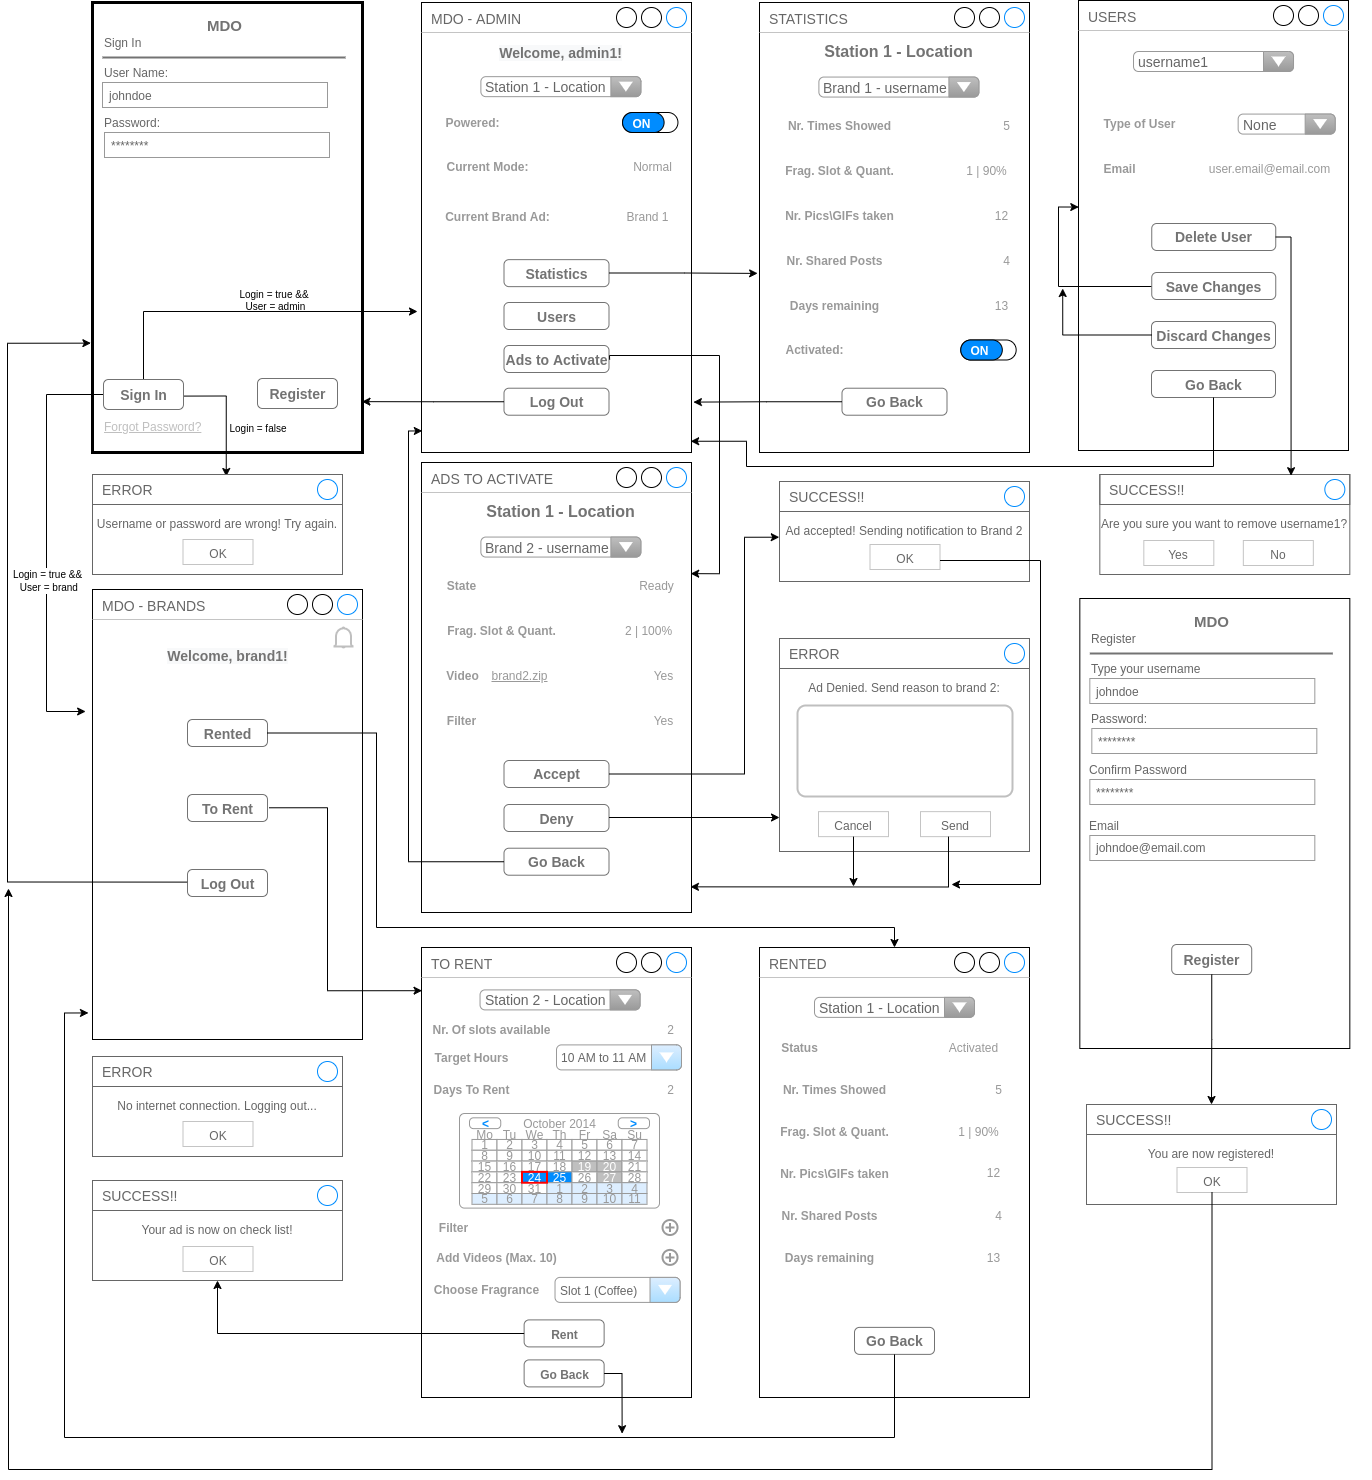
\includegraphics[width=0.9\columnwidth]{./img/user-mockups-rc.png}
  \caption{User mockups: remote client}%
\label{fig:user-mockups-rc}
\end{figure}

\subsubsection{Events}
\label{sec:events-1}
Table~\ref{tab:events-rc} presents the most relevant events for the Local system, categorizing them by their source and
synchronism and linking it to the system’s intended response.

%
\begingroup
\renewcommand{\arraystretch}{0.7} % Default value: 1
% Please add the following required packages to your document preamble:
% \usepackage{booktabs}
% \usepackage{graphicx}
\begin{table}[]
\centering
\caption{Events: remote client}
\label{tab:events-rc}
\resizebox{\textwidth}{!}{%
\begin{tabular}{@{}llll@{}}
\toprule
\textbf{Event} &
  \textbf{System response} &
  \textbf{Source} &
  \textbf{Type} \\ \midrule
Login &
  \begin{tabular}[c]{@{}l@{}}The system verifies if the user credentials\\ are correct and what type of user is and\\ asks for data from databases\end{tabular} &
  User &
  Asynchronous \\ \midrule
Verify internet connection &
  Periodically verify internet connection &
  Remote Client &
  Synchronous \\ \midrule
Statistics &
  \begin{tabular}[c]{@{}l@{}}Request to the Remote Server all the\\  information to show statistics from \\ all stations and brands\end{tabular} &
  User (Admin) &
  Asynchronous \\ \midrule
Accept/Deny ad &
  \begin{tabular}[c]{@{}l@{}}Send information to the Remote \\ Server if the ad is either accepted\\ or denied and if so, why\end{tabular} &
  User (Admin) &
  Asynchronous \\ \midrule
Power On/Off Station &
  \begin{tabular}[c]{@{}l@{}}Send command to Remote Server\\  to Power On/Off a certain station\end{tabular} &
  User (Admin) &
  Asynchronous \\ \midrule
Rented &
  \begin{tabular}[c]{@{}l@{}}Request to the Remote Server all the\\  information to show statistics from \\ all stations the brand rented\end{tabular} &
  User (Brand) &
  Asynchronous \\ \midrule
Rent &
  \begin{tabular}[c]{@{}l@{}}Send to the Remote Server all the \\ information of rent from the brand, \\ all the videos and the filter\end{tabular} &
  User (Brand) &
  Asynchronous \\ \midrule
Forgot Password &
  \begin{tabular}[c]{@{}l@{}}Send e-mail to the user that has \\ forgotten his password\end{tabular} &
  User &
  Asynchronous \\ \bottomrule
\end{tabular}%
}
\end{table}
%
%
%
\subsubsection{Use cases}
\label{sec:use-cases-1}
%
Fig.~\ref{fig:use-cases-rc} depicts the use cases diagram for the \texttt{Remote Client}, describing how the system should respond under various conditions to a request from one of the stakeholders to deliver a specific
goal.

The \texttt{Admin} and the \texttt{Brand} interact with the \texttt{Remote Client} and this last interacts with the \texttt{Remote Server} to process commands, such as query databases or power on/off machines.

The \texttt{Admin} can Manage the Station, which includes Power On/Off Station, Manage Ads to Activate and Enable/Disable an Ad.
It can also manage users, removing or modifying them. All these use cases are processed from the \texttt{Remote Client} and are requested to the \texttt{Remote Server}.

The \texttt{Brand} can see Rented Ads, Rent Ads, See notifications and register. All these cases are also processed from the \texttt{Remote Client} and are requested to the \texttt{Remote Server}.

There are some use cases that are common to the  \texttt{Admin} and to the \texttt{Brand}: Login and Logout.


\begin{figure}[htb!]
\centering
    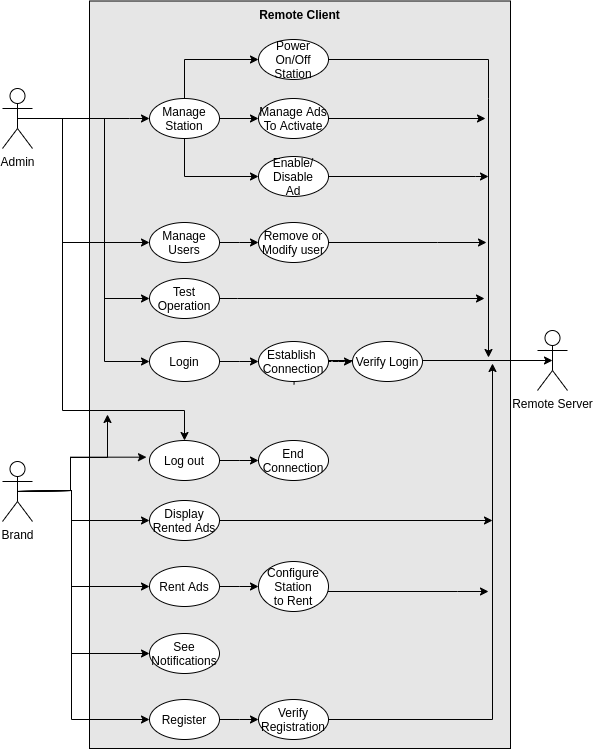
\includegraphics[width=0.6\columnwidth]{./img/use-cases-rc.png}
  \caption{Use cases: remote client}%
\label{fig:use-cases-rc}
\end{figure}


\subsubsection{Dynamic operation}
\label{sec:dyn-oper-1}

Fig.~\ref{fig:state-mach-rc} depicts the state machine diagram for the
\texttt{Remote Client}, illustrating its dynamic behavior. There are two main
states:
\begin{item-c}
\item \emph{\texttt{Initialization}}: the app is initialized. The settings are loaded and if invalid they are restored. The WiFi communication is setup, signaling the communication status and if valid, an \gls{ip} address is returned.
\item \emph{\texttt{Execution}}: after the initialization is successful, the system goes into the \texttt{Execution} macro composite state with several concurrent activities, modeled as composite states too. However, it should be noted that there is only one actual state for the device, although at the perceivable time scale they appear to happen simultaneously. These activities are communication management (\texttt{Comm Manager}), interface management (\texttt{\gls{ui} Engine}) and application manager (\texttt{App Manager}), and are executed forever until system's power off. They are detailed next.
\end{item-c}

%
\begin{figure}[htb!]
\centering
    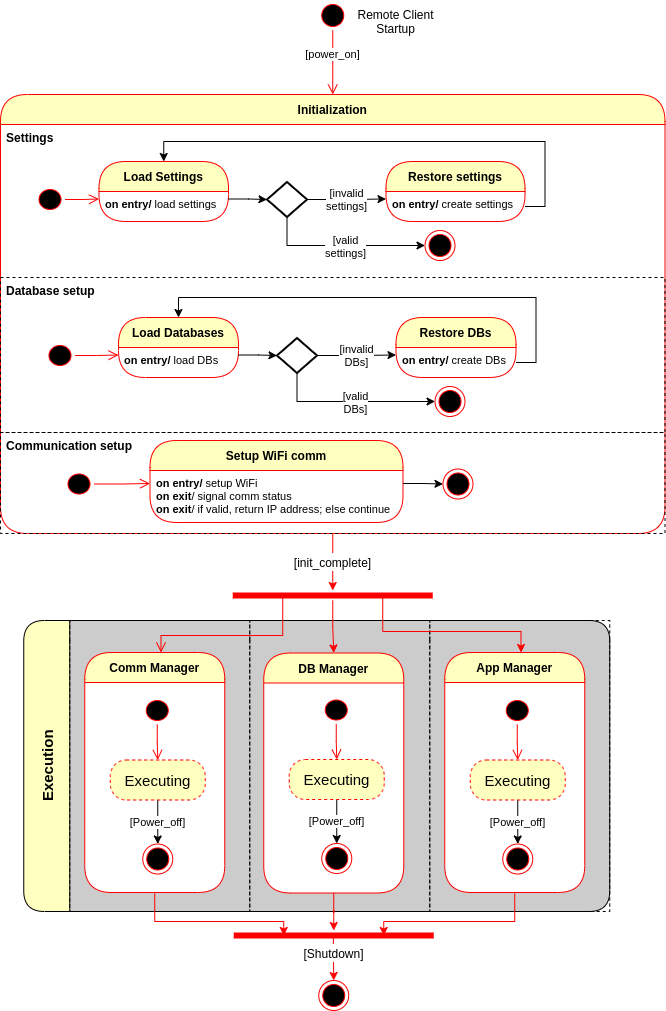
\includegraphics[width=0.9\columnwidth]{./img/state-mach-rc.png}
  \caption{State Machine Diagram: remote client}%
\label{fig:state-mach-rc}
\end{figure}
%

\paragraph{\emph{Communication Manager}}
Fig.~\ref{fig:state-mach-local-comm} depicts the state machine diagram for the
\texttt{Comm Manager} component. Upon successful initialization the
\texttt{Comm Manager} goes to \texttt{Idle}, listening for incoming
connections. When a remote node tries to connects, it makes a connection request
which can be accepted or denied. If the connection is accepted and the node
authenticates successfully the \texttt{Comm Manager} is ready for bidirectional
communication. When a message is received from the remote node, it is written to
\texttt{TX msg queue} and the \texttt{Supervisor} is notified. When a message
must be sent to the remote, it is read from the \texttt{TX msg queue} and sent
to the recipient. If the connection goes down, it is restarted, going into
\texttt{Idle} state again.

\begin{figure}[htb!]
\centering
    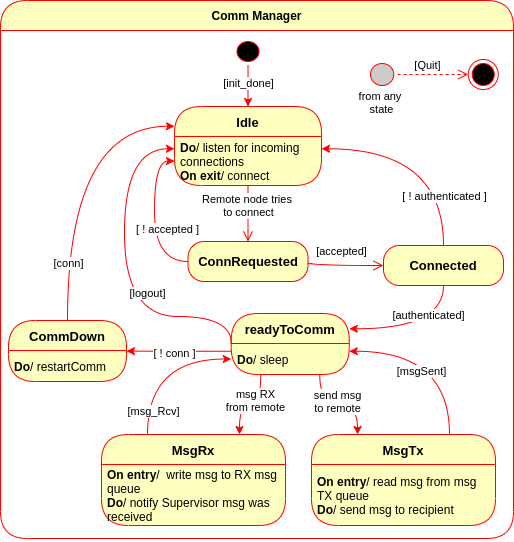
\includegraphics[width=0.5\columnwidth]{./img/state-mach-rc-comm.png}
  \caption{State Machine Diagram: remote client - Communication Manager}%
\label{fig:state-mach-rc-comm}
\end{figure}
%

\paragraph{\emph{App Manager}}
Fig.~\ref{fig:state-mach-rc-app-manag} depicts the state machine diagram for the
\texttt{App Manager} component.
Upon successful initialization the
\texttt{App Manager} goes to \texttt{Login}, waiting for some action. 

A user can try to register pressing the 'Register' button which leads to \texttt{Register} state, if it registers well, it come back again to \texttt{Login} state. 
If the 'Login' button is pressed, the system goes to \texttt{Validation} state, where it validates wether the user is an admin or a brand.

If it's \texttt{Admin Mode} state, the user has several states where it can see statistics (\texttt{Statistics}), manage all users (\texttt{Users}) and manage all ads to actvivate (\texttt{Ads To Activate}).
If it's \texttt{Brand Mode} state, the user has several states where it can see all his ads (\texttt{Rented}), see notifications and messages (\texttt{Main Menu}) and rent new ads (\texttt{To Rent}). 
Each two of the states end pressing the 'Log Out' button, which redirects to \texttt{Login}  state.

In any state it can occur the unexpected quit of the application. If that happens, then all state machines come to an end.  

%
\begin{figure}[htb!]
\centering
    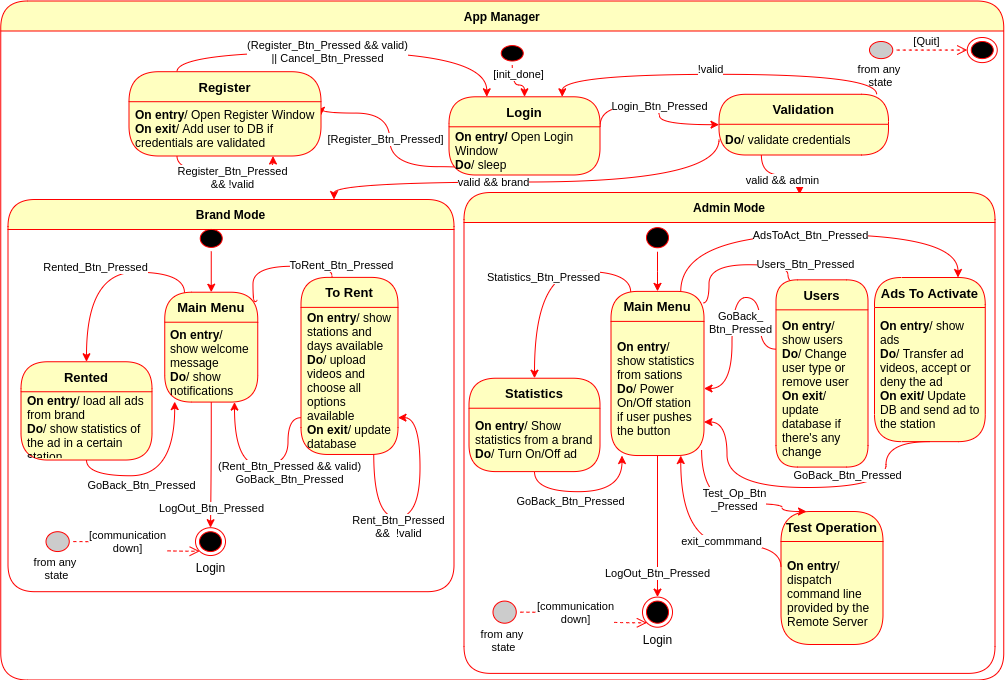
\includegraphics[width=0.9\columnwidth]{./img/state-mach-rc-app-manag.png}
  \caption{State Machine Diagram: remote client - App Manager}%
\label{fig:state-mach-rc-app-manag}
\end{figure}
%
%
%

\subsubsection{Flow of events}
\label{sec:flow-events-1}
The flow of events throughout the system is described using a sequence diagram, comprising the interactions between the most relevant system's entities.
It is usually pictured as the visual representation of an use case. The main sequence diagrams are illustrated next.

\begin{figure}[htb!]
\centering
    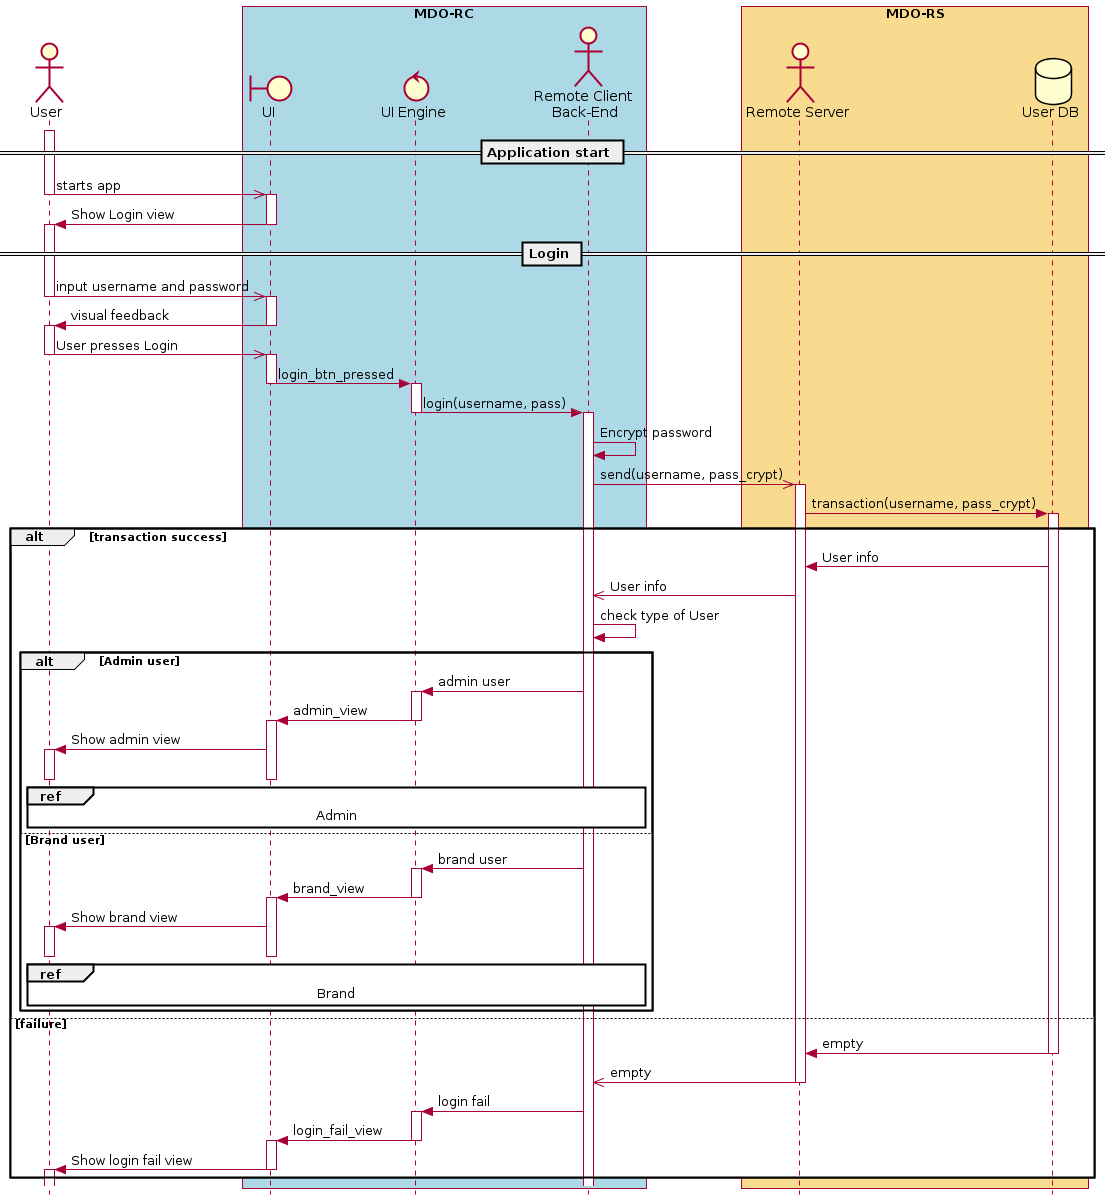
\includegraphics[width=1\columnwidth]{./img/seq-rc-login.png}
  \caption{Sequence Diagram: remote client - Login}%
\label{fig:seq-rc-login}
\end{figure}

\begin{figure}[htb!]
\centering
    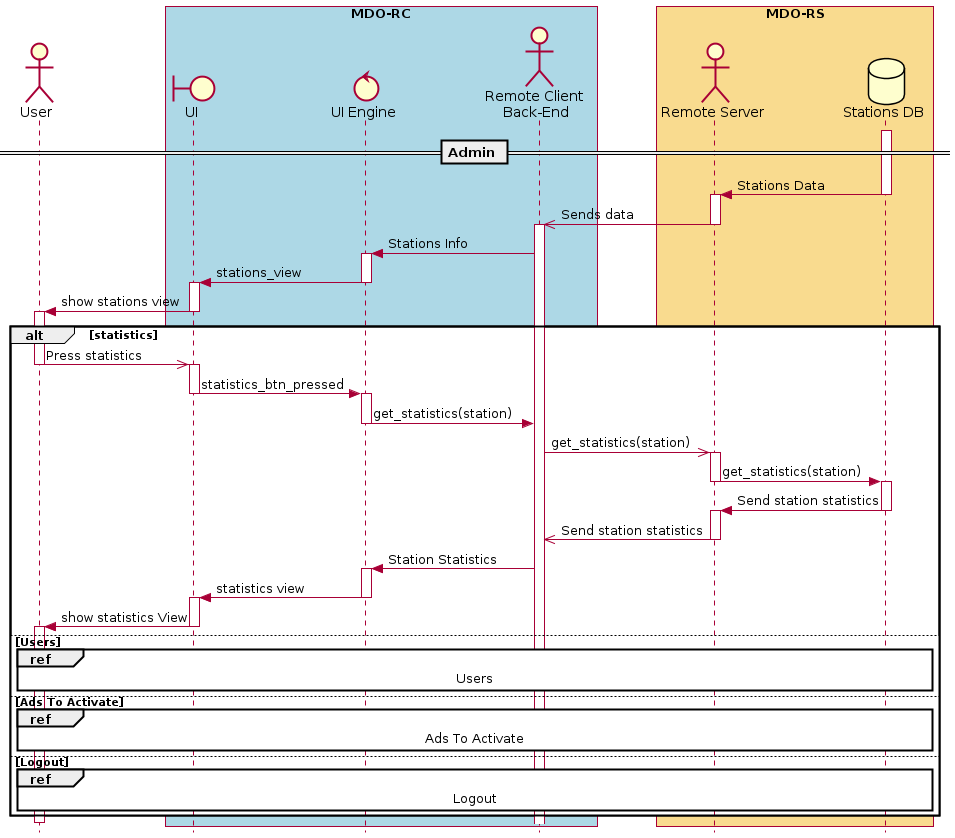
\includegraphics[width=1\columnwidth]{./img/seq-rc-admin-statistics.png}
  \caption{Sequence Diagram: remote client - admin statistics}%
\label{fig:seq-rc-admin-statistics}
\end{figure}

\begin{figure}[htb!]
\centering
    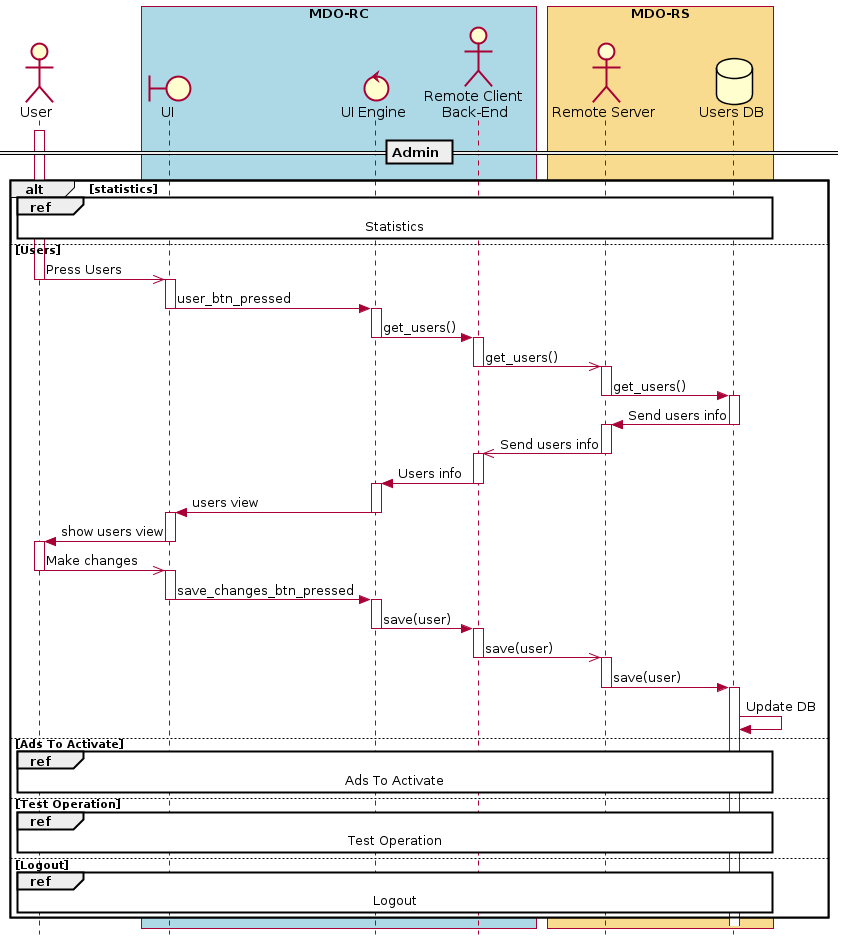
\includegraphics[width=1\columnwidth]{./img/seq-rc-admin-users.png}
  \caption{Sequence Diagram: remote client - admin users}%
\label{fig:seq-rc-admin-users}
\end{figure}

\begin{figure}[htb!]
\centering
    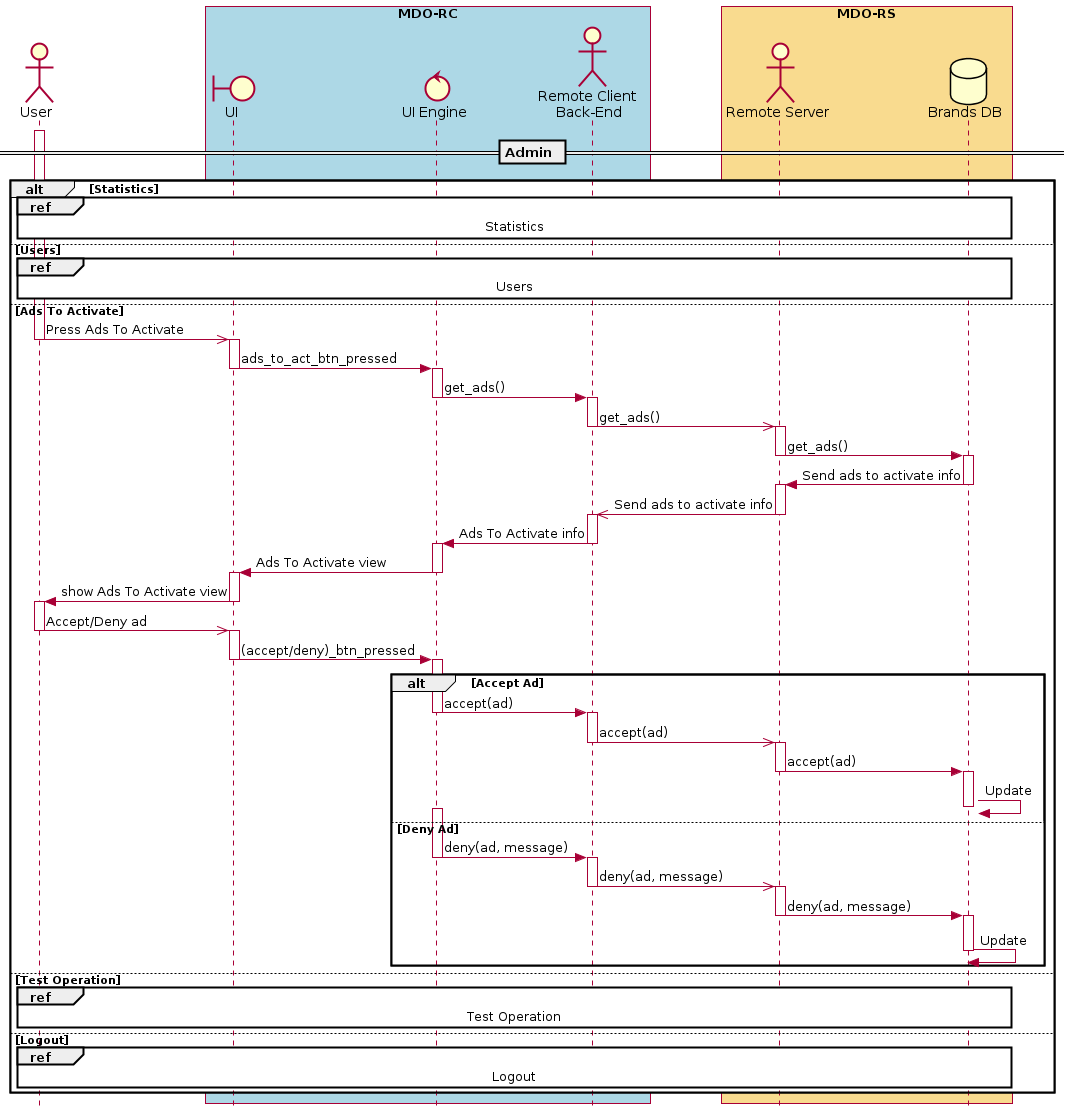
\includegraphics[width=1\columnwidth]{./img/seq-rc-admin-ads-to-act.png}
  \caption{Sequence Diagram: remote client - admin ads to activate}%
\label{fig:seq-rc-admin-ads-to-act}
\end{figure}

\begin{figure}[htb!]
\centering
    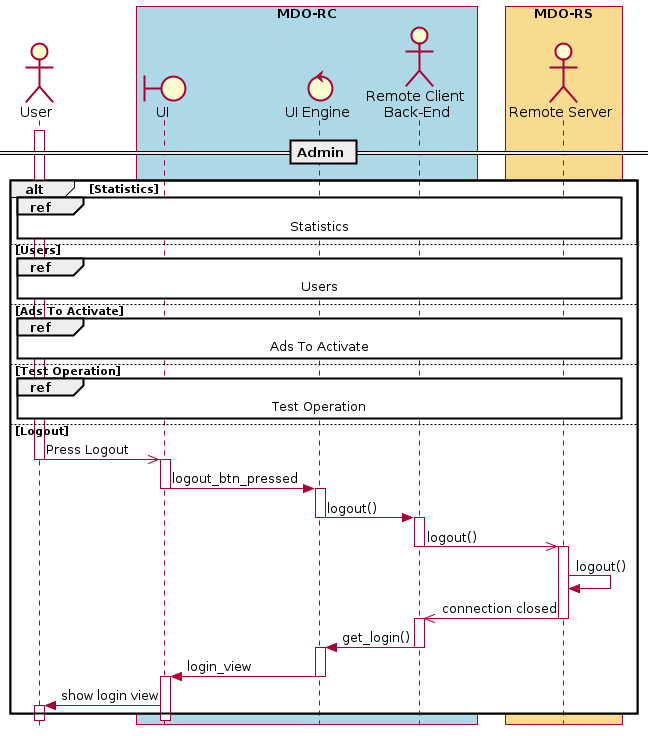
\includegraphics[width=0.7\columnwidth]{./img/seq-rc-admin-logout.png}
  \caption{Sequence Diagram: remote client - admin logout}%
\label{fig:seq-rc-admin-logout}
\end{figure}

As it can be seen, the user interacts with the \texttt{\gls{ui}}, then this last interacts with the \texttt{\gls{ui} Engine}, interacting with the \texttt{Remote Client Back-End} in order to process and execute all the information and commands needed. 
There's an alternate way to go to the user, that's because on the authentication the \texttt{Remote Client Back-End} will discover if the user is an \texttt{Admin} or a \texttt{Brand}.
On both cases, it shows its main menu and it can end the sequence through the 'Logout'.
In each one of the cases there's alternative sequences to occur, depending in what the \texttt{User} decides to do.
Also, in each alternative choice, the \texttt{Remote Client} can interact with different \texttt{Databases}, either to update them or to ask some info.

%%% Local Variables:
%%% mode: latex
%%% TeX-master: "../../../dissertation"
%%% End:
